% Vía B: modelo económico propio. Formato del curso.
\documentclass[11pt]{article}
\usepackage[utf8]{inputenc}
\IfFileExists{lmodern.sty}{\usepackage[T1]{fontenc}\usepackage{lmodern}}{\usepackage[OT1]{fontenc}}
\IfFileExists{spanish.ldf}{\usepackage[spanish,es-nodecimaldot]{babel}}{\usepackage[english]{babel}}
\usepackage[margin=1in]{geometry}
\usepackage[expansion=false]{microtype}
\usepackage{amsmath,amssymb,amsthm}
\usepackage{booktabs,graphicx}
\usepackage{xcolor}
\usepackage[round]{natbib}
\usepackage[colorlinks=true,allcolors=blue!50!black]{hyperref}
\newtheorem{assumption}{Supuesto}
\renewcommand{\theassumption}{A\arabic{assumption}}
\newtheorem{proposition}{Proposición}
\renewcommand{\proofname}{Demostración}
\newcommand{\KA}{K^{A}}
\newcommand{\KV}{K^{V}}
\newcommand{\kA}{\kappa^{A}}
\newcommand{\kV}{\kappa^{V}}
\title{Fricciones de ejecución, intensidad óptima y condición de sobrecosto en proyectos municipales}
\author{Isis Milagros Roque Tinta\thanks{Universidad del Pacífico. Vía B: modelo teórico motivado por una propuesta anterior de tesis sobre pobreza distrital y ejecución de proyectos. Repositorio: \url{https://github.com/isisroquet-mi/ai-project}.}}
\date{25 de noviembre de 2026}
\begin{document}
\renewcommand{\abstractname}{Resumen}
\renewcommand{\refname}{Referencias}
\renewcommand{\proofname}{Demostración}
\maketitle
\begin{abstract}
\noindent Se estudia cómo la dificultad de acelerar un proyecto municipal afecta su intensidad, duración y costo, y cuándo el costo realizado supera al previsto. El municipio ejecuta una obra de alcance fijo y elige una intensidad constante para minimizar el costo de permanencia y de aceleración. Si el gasto por período y la fricción son positivos, existe un único óptimo global: una mayor fricción reduce la intensidad y aumenta la duración y el costo. Para el mismo proyecto, con costo base y gasto periódico comunes a la previsión y la ejecución, hay sobrecosto si y solo si la fricción efectiva supera la anticipada. Los signos distritales dependen de supuestos sobre pobreza y capacidad municipal, sin interpretación causal estimada. SymPy y comprobaciones numéricas reproducen identidades y figuras. La formalización Lean disponible acredita solo el mínimo global único; los demás resultados aún no están formalizados.
\end{abstract}

\section{Introducción}\label{sec:intro}
Una municipalidad puede mantener abierta una obra durante más tiempo o asignar recursos para avanzar a mayor ritmo. La primera alternativa prolonga los gastos de administración y coordinación; la segunda exige organizar personal, insumos y supervisión de manera más intensa. Cuando esas tareas resultan más difíciles de lo previsto, el costo de una obra concluida puede diferir del presupuesto con el que se la comparaba. Distinguir entre la dificultad de ejecutar y la calidad de la previsión resulta esencial al analizar duración y variaciones de costos.

La pregunta de investigación que motivó este ejercicio teórico se refería a la relación entre pobreza distrital, velocidad de ejecución y variación de costos de proyectos locales en el Perú. Este artículo, elaborado por la vía B del curso, formula una pregunta más acotada: ¿cómo cambia la intensidad elegida por un municipio cuando ejecutar se vuelve más difícil y cuándo se produce un sobrecosto con respecto a la previsión? El modelo se inspira en aquella propuesta anterior de tesis, que no constituye una prueba empírica de sus mecanismos y debe distinguirse de la línea posterior de investigación de la autora sobre modalidades de ejecución.

Se representa la dificultad mediante una fricción positiva, $\kappa$, que multiplica el costo de acelerar. Con un gasto positivo $F$ por período, el municipio elige la intensidad $e>0$ que minimiza $K(e;\kappa)=M+F/e+\kappa e/2$, donde $M$ es un costo base común a las alternativas. El resultado es $e^*=\sqrt{2F/\kappa}$, una duración $T^*=\sqrt{\kappa/(2F)}$ y un costo $K^*=M+\sqrt{2F\kappa}$. Si el presupuesto se calculó con una fricción prevista $\kV>0$ y, al iniciar la obra, la fricción efectiva es $\kA>0$, entonces el sobrecosto medido por $R=\log(\KA/\KV)$ es positivo exactamente cuando $\kA>\kV$, siempre que se compare el mismo proyecto con los mismos $M$ y $F$.

La contribución consiste en reunir una decisión continua de intensidad, condiciones transparentes de heterogeneidad distrital y una comparación precisa entre costo previsto y efectivo dentro de un mecanismo pequeño. \citet{mohammadi2022} ya optimizan el intercambio entre tiempo y costo bajo incertidumbre, de modo que este artículo no reclama la invención de ese intercambio. Frente a la evidencia peruana reciente de \citet{julca2025}, que identifica riesgos de retrasos y sobrecostos en obras de agua y saneamiento, aquí se obtiene una condición analítica para la variación de costo y se separa el costo de ejecutar de la fricción incorporada en la previsión. Asimismo, los hallazgos de \citet{eliasson2025} sobre la importancia de la etapa de estimación motivan especificar cuándo se fija el costo de referencia; el modelo no reproduce sus procesos de selección ni de revisión del diseño.

Tras revisar los antecedentes directamente relacionados con capacidad pública, previsión y gestión de proyectos, se exponen las primitivas y el orden de decisiones, se demuestran dos proposiciones y se desarrolla una extensión de anticipación parcial. Las simulaciones comprueban identidades y signos en escenarios ilustrativos, antes de discutir los límites de la correspondencia con medidas administrativas.

\section{Literatura relacionada}\label{sec:literatura}
\citet{loayza2014} estudian la capacidad de los municipios peruanos para ejecutar los presupuestos que se les asignan. Su análisis combina cuentas fiscales con características municipales y distingue asignación presupuestaria, capacidad local, necesidades y economía política. En la sección de resultados encuentran que la capacidad y la escala presupuestaria importan para el gasto; también observan, condicional a sus controles, que municipalidades con mayor pobreza ejecutan una fracción mayor de su presupuesto asignado. La unidad de observación y el resultado de ese estudio no equivalen a la duración ni al costo final de una obra individual. Además, el signo positivo de la pobreza en la fracción gastada advierte que las necesidades pueden impulsar el gasto por un canal distinto del costo de acelerar. La hipótesis $\kappa_p>0$ que se utilizará más adelante constituye, por ello, una restricción estructural para estudiar un mecanismo y no una conclusión empírica atribuible a \citet{loayza2014}.

El intercambio entre tiempo y costo pertenece a una literatura amplia de gestión de proyectos. \citet{mohammadi2022}, en un artículo publicado en \emph{Journal of Industrial and Systems Engineering}, estudian una optimización bajo incertidumbre con simulación Monte Carlo, un algoritmo de búsqueda y una restricción financiera asociada al sobregiro. Su problema considera actividades y fuentes de incertidumbre que este artículo omite. Por su parte, \citet{gurara2020} relacionan la ampliación de la inversión pública con costos unitarios de proyectos viales en países en desarrollo y encuentran una asociación no lineal compatible con límites de absorción. Ese texto se cita como \emph{IMF Working Paper} WP/20/48, es decir, como documento de trabajo y no como artículo de revista. Su fricción de capacidad se refiere a la escala de inversión y no identifica una derivada de la pobreza distrital sobre el costo de acelerar una obra municipal.

Para distinguir el presupuesto del costo realizado, \citet{flyvbjerg2002}, en un artículo publicado en \emph{Journal of the American Planning Association} cuya copia disponible también circula como prepublicación, documentan la subestimación de costos en 258 proyectos de transporte. \citet{eliasson2025} siguen estimaciones de infraestructura sueca desde la planificación hasta el cierre y muestran que el resultado de la comparación depende de la etapa en que se toma la estimación: buena parte del aumento ocurre antes de la decisión final de construir. Estos hallazgos impiden tratar cualquier monto inicial como si se basara en la misma información disponible al comienzo de la ejecución. En el modelo, $\KV$ es un costo calculado antes de conocer completamente $\kA$; su interpretación empírica exige identificar el momento presupuestario concreto y mantenerlo fijo en las comparaciones.

La evidencia más cercana en unidades de proyecto incluye a \citet{issa2022}, que estudian costo y duración previstos frente a realizados en 46 proyectos viales municipales de Palestina. Los autores documentan variaciones relacionadas con subestimación, retrasos de contratistas y órdenes que modifican el alcance, entre otros factores. En el Perú, \citet{julca2025} analizan documentación de 318 proyectos de agua y saneamiento e identifican, entre los riesgos frecuentes, aprobaciones tardías de cambios, información de terreno inexacta, estimaciones de diseño imprecisas y disponibilidad de terrenos. \citet{ariza2025} proponen estimaciones probabilísticas de costo y plazo para tres proyectos viales peruanos y muestran la relevancia práctica de la incertidumbre previa. Esos trabajos motivan separar información inicial y dificultades realizadas, aunque las modificaciones de alcance que describen quedan fuera de la comparación estricta del mismo proyecto adoptada aquí.

\section{Modelo}\label{sec:modelo}
\subsection{Primitivas, trabajo y costo}
El agente es un gobierno municipal que ejecutará una obra individual. El trabajo representa la cantidad de avance físico necesario para completarla, no las horas trabajadas por un empleado ni una medida observada de gasto financiero. La unidad de ese trabajo se normaliza a $Q=1$ y el proyecto comienza en $t=0$. Si $e$ es el avance por unidad de tiempo y permanece constante hasta la terminación, entonces $Q=eT=1$ y la fecha de culminación coincide con la duración $T(e)=1/e$.

\begin{assumption}[Proyecto y decisión]\label{ass:proyecto}
El proyecto se realiza y mantiene alcance y calidad fijos. El municipio estudia cómo ejecutarlo, no si conviene iniciarlo, y minimiza su costo de implementación. Cualquier beneficio $B$ es independiente de la intensidad $e$, de modo que maximizar $B-K(e;\kappa)$ y minimizar $K(e;\kappa)$ son problemas equivalentes.
\end{assumption}
\begin{assumption}[Intensidad constante]\label{ass:intensidad}
En el inicio de la ejecución se elige una sola intensidad $e\in(0,\infty)$, que se mantiene hasta terminar el proyecto. No hay pausas, revisión de $e$, trayectoria $e(t)$ ni restricción superior de capacidad.
\end{assumption}
\begin{assumption}[Costos y positividad]\label{ass:costos}
El costo base $M\geq0$ se paga por el proyecto; $F>0$ es un gasto fijo por período mientras la obra está abierta; y $\kappa>0$ mide la dificultad de acelerar. Durante una ejecución concreta estos parámetros son constantes. El costo de intensidad por período es $\kappa e^2/2$.
\end{assumption}

El municipio minimiza el costo acumulado hasta la culminación, sujeto al trabajo por completar:
\begin{equation}\label{eq:problema}
 \min_{e>0}\;K(e;\kappa)
 =M+\int_0^{T(e)}\left(F+\frac{\kappa e^2}{2}\right)\,dt,
 \qquad eT(e)=1.
\end{equation}
La letra $t$ es solamente la variable de integración; $F$, $e$ y $\kappa$ no cambian dentro del intervalo $[0,1/e]$. Al sustituir $T(e)=1/e$ e integrar se obtiene
\begin{equation}\label{eq:costo}
 K(e;\kappa)=M+\left(F+\frac{\kappa e^2}{2}\right)\frac1e
 =M+\frac Fe+\frac{\kappa e}{2}.
\end{equation}
Una mayor intensidad reduce los períodos durante los cuales se paga $F$, aunque encarece el esfuerzo de acelerar que se acumula hasta terminar. El término $M$ desplaza el nivel de costo sin alterar la intensidad óptima.

\subsection{Heterogeneidad e información}
\begin{assumption}[Fricción local]\label{ass:hetero}
En el dominio relevante, la fricción efectiva es $\kA=\kappa(p,C)>0$, diferenciable respecto de la incidencia de pobreza distrital predeterminada $p$ y de una medida de capacidad municipal $C$, con $\kappa_p:=\partial\kappa/\partial p>0$ y $\kappa_C:=\partial\kappa/\partial C<0$. Las comparaciones respecto de $p$ o $C$ mantienen fijos $M$, $F$ y la otra característica distrital.
\end{assumption}
El supuesto \ref{ass:hetero} recoge la posibilidad de que restricciones locales eleven la coordinación necesaria para avanzar a un ritmo dado, y de que personal y procedimientos municipales reduzcan ese esfuerzo. No se presupone que la pobreza sea la única determinante de $\kappa$ ni se infiere el signo de $\kappa_p$ directamente de la evidencia sobre ejecución presupuestaria. En particular, la asociación encontrada por \citet{loayza2014} para la fracción de presupuesto gastada puede coexistir con un canal de fricción distinto o indicar que el supuesto requiere revisión empírica.

\begin{assumption}[Previsión comparable]\label{ass:prevision}
Antes de ejecutar, una estimación con información incompleta utiliza una fricción prevista $\kV>0$ y proyecta la intensidad y el costo mínimos de la misma obra. Al comenzar la ejecución se conoce $\kA>0$, se elige $e^A$ una sola vez y se realiza la obra. Entre la previsión y la realización se mantienen el alcance, la calidad, $M$ y $F$; no hay cambios de precios, revisión del presupuesto de referencia ni selección de obras que finalmente no se ejecutan.
\end{assumption}
Esta sincronización distingue una proyección de una elección realizada. La estimación previa puede diferir de la dificultad efectiva porque ciertos requerimientos de terreno, coordinación o abastecimiento se conocen mejor al comenzar la obra; el modelo no precisa una distribución de información ni presupone que el municipio desconozca por completo su propia capacidad. La proyección $e^V$ es el ritmo que habría minimizado el costo bajo $\kV$, no una intensidad vinculante elegida con anticipación. El momento del presupuesto es anterior al inicio; al comenzar se selecciona $e^A$ y durante la ejecución no se vuelve a optimizar.

\section{Resultados y demostraciones}\label{sec:resultados}
\subsection{Intensidad, duración y costo}
\begin{proposition}[Óptimo único y signos de la fricción]\label{prop:uno}
Bajo \ref{ass:proyecto}--\ref{ass:costos}, para todo $M\geq0$, $F>0$ y $\kappa>0$, el problema \eqref{eq:problema} tiene un único minimizador global en $e>0$, y sus resultados son
\begin{equation}\label{eq:optimo}
 e^*(\kappa)=\sqrt{\frac{2F}{\kappa}},\qquad
 T^*(\kappa)=\sqrt{\frac{\kappa}{2F}},\qquad
 K^*(\kappa)=M+\sqrt{2F\kappa}.
\end{equation}
Con $M$ y $F$ fijos, $e^*_{\kappa}<0$, $T^*_{\kappa}>0$ y $K^*_{\kappa}>0$. Si también se cumple \ref{ass:hetero}, una mayor $p$ reduce $e^*$ y aumenta $T^*$ y $K^*$; una mayor $C$ produce los signos opuestos, manteniendo fijos los parámetros y la otra característica local.
\end{proposition}
\begin{proof}
La derivada del costo \eqref{eq:costo} respecto de la intensidad es $K_e=-F/e^2+\kappa/2$, por lo que la condición de primer orden $K_e=0$ equivale a $e^2=2F/\kappa$. Como $F$ y $\kappa$ son positivos y $e>0$, el único candidato interior es $q=\sqrt{2F/\kappa}>0$. La segunda derivada $K_{ee}=2F/e^3>0$ identifica un mínimo local; para establecer también globalidad y unicidad se usa la identidad $F=\kappa q^2/2$. En efecto, para todo $e>0$,
\begin{align}\label{eq:brecha}
 K(e;\kappa)-K(q;\kappa)
 &=\frac Fe+\frac{\kappa e}{2}-\frac Fq-\frac{\kappa q}{2}\notag\\
 &=\frac{\kappa q^2}{2e}+\frac{\kappa e}{2}-\kappa q
 =\frac{\kappa}{2e}(e-q)^2\geq0.
\end{align}
El último término se anula exactamente en $e=q$ porque $\kappa/(2e)>0$; por tanto, $q$ alcanza el mínimo y es el único minimizador global. Al sustituir $q$ en $T(e)=1/e$ y \eqref{eq:costo} se obtiene \eqref{eq:optimo}. La diferenciación directa, válida para $F,\kappa>0$, da
\begin{equation}\label{eq:derivadas}
 e^*_{\kappa}=-\frac{\sqrt{2F}}{2\kappa^{3/2}}<0,\qquad
 T^*_{\kappa}=\frac{1}{2\sqrt{2F\kappa}}>0,\qquad
 K^*_{\kappa}=\sqrt{\frac{F}{2\kappa}}>0.
\end{equation}
Bajo \ref{ass:hetero}, la regla de la cadena establece para $x\in\{p,C\}$ que $e_x^*=e_{\kappa}^*\kappa_x$, $T_x^*=T_{\kappa}^*\kappa_x$ y $K_x^*=K_{\kappa}^*\kappa_x$. Los signos se siguen de \eqref{eq:derivadas}, $\kappa_p>0$ y $\kappa_C<0$.
\end{proof}
La comparación respecto de la pobreza designa una variación hipotética de $p$ que, por \ref{ass:hetero}, eleva $\kappa$ sin alterar $C$, $M$ ni $F$. No se afirma que dos distritos observados difieran solamente en pobreza, ni que $\kappa_p$ haya sido estimado. La consecuencia teórica sobre $K^*$ se refiere al nivel de costo óptimo, que todavía no informa si el costo supera un presupuesto particular.

\subsection{Condición exacta de sobrecosto}
Bajo \ref{ass:prevision}, aplíquese la solución \eqref{eq:optimo} a las fricciones de las dos etapas. El monto previsto y el costo realizado del mismo proyecto son
\begin{equation}\label{eq:etapas}
 e^V=\sqrt{\frac{2F}{\kV}},\quad T^V=\frac1{e^V},\quad
 \KV=M+\sqrt{2F\kV};\qquad
 e^A=\sqrt{\frac{2F}{\kA}},\quad T^A=\frac1{e^A},\quad
 \KA=M+\sqrt{2F\kA}.
\end{equation}
Se define la variación logarítmica $R:=\log(\KA/\KV)$. Ambas cantidades son estrictamente positivas aunque $M$ pueda ser cero, pues $F$, $\kA$ y $\kV$ son positivos. Así, $R$ está definido tanto para sobrecosto como para igualdad y costo menor que el previsto.
\begin{proposition}[Tres signos de la variación de costos]\label{prop:dos}
Bajo \ref{ass:proyecto}--\ref{ass:costos} y \ref{ass:prevision}, para el mismo proyecto con $M\geq0$, $F>0$ y $\kA,\kV>0$,
\begin{equation}\label{eq:signos}
 \operatorname{sgn}(R)=\operatorname{sgn}(\KA-\KV)
 =\operatorname{sgn}(\kA-\kV).
\end{equation}
En consecuencia, $R>0$ si y solo si $\kA>\kV$; $R=0$ si y solo si $\kA=\kV$; y $R<0$ si y solo si $\kA<\kV$.
\end{proposition}
\begin{proof}
Por \eqref{eq:etapas}, la diferencia de costos cancela el término base $M$ y satisface
\begin{equation}\label{eq:resta}
 \KA-\KV=\sqrt{2F}\bigl(\sqrt{\kA}-\sqrt{\kV}\bigr).
\end{equation}
Como $F>0$, el factor $\sqrt{2F}$ es positivo; como las fricciones son positivas, la raíz cuadrada es estrictamente creciente. Por tanto, $\KA-\KV$ y $\kA-\kV$ tienen el mismo signo, incluido el caso de igualdad. Finalmente, $\KA,\KV>0$ permite escribir $R=\log(\KA/\KV)$, y el logaritmo es estrictamente creciente con $\log 1=0$. De ahí que $R$ sea positivo, cero o negativo exactamente cuando $\KA/\KV$ sea mayor, igual o menor que uno, lo que equivale a comparar $\KA$ con $\KV$. Esto prueba \eqref{eq:signos} y los tres casos.
\end{proof}
La condición no dice que un proyecto de fricción elevada siempre presente sobrecosto: una obra difícil puede ajustarse a un presupuesto igualmente alto si la dificultad fue anticipada. Tampoco permite reemplazar $\kA>\kV$ por $\kappa_p>0$: la primera compara niveles entre etapas y la segunda expresa una derivada hipotética respecto de una característica distrital.

\subsection{Anticipación parcial y variación respecto de la pobreza}\label{sec:anticipacion}
Para ilustrar qué cambia cuando una previsión incorpora mejor la dificultad local, considérese una fricción genérica $\bar\kappa>0$ y el índice exógeno $\lambda\in[0,1]$ definido por
\begin{equation}\label{eq:lambda}
 \kV(\lambda)=\lambda\kA+(1-\lambda)\bar\kappa.
\end{equation}
En $\lambda=0$ la previsión utiliza únicamente $\bar\kappa$; para $0<\lambda<1$ incorpora parte de la fricción efectiva; y en $\lambda=1$ la anticipa completamente. El índice no es una decisión del municipio ni se deriva de expectativas racionales. Por positividad de $\kA$ y $\bar\kappa$, la combinación \eqref{eq:lambda} es positiva en todo el intervalo.

Con $\kA$, $M$ y $F$ fijos, la intensidad realizada $e^A$ y el costo realizado $\KA$ no varían con $\lambda$, mientras que la derivada del indicador es
\begin{equation}\label{eq:r_lambda}
 \frac{\partial R}{\partial\lambda}
 =-\frac{\sqrt{F/(2\kV(\lambda))}}{\KV(\lambda)}
   (\kA-\bar\kappa).
\end{equation}
La expresión resulta de derivar $R=\log\KA-\log\KV(\lambda)$: la primera parte es constante y la derivada de $\KV$ respecto de $\kV$ vale $\sqrt{F/(2\kV)}$. El factor anterior a $\kA-\bar\kappa$ es estrictamente negativo. Si $\kA>\bar\kappa$, una mayor anticipación disminuye un $R$ positivo para $\lambda<1$; si $\kA<\bar\kappa$, eleva un $R$ negativo. Cuando $\kA=\bar\kappa$, $R=0$ para cualquier $\lambda$, y en los otros casos $R(1)=0$. El resultado describe una previsión que se acerca al costo realizado manteniendo fija la dificultad de ejecutar, no una obra que se abarata por aumentar $\lambda$.

La derivación manuscrita disponible de la autora examina otra distinción: si la previsión también varía con la pobreza, no basta con suponer $\kappa_p^A>0$ para concluir que $R_p>0$. Si ambas funciones $\kA(p)$ y $\kV(p)$ son positivas y diferenciables, con $M$ y $F$ fijos, la regla de la cadena conduce a
\begin{equation}\label{eq:rp}
 R_p=\frac{(\KA)_p}{\KA}-\frac{(\KV)_p}{\KV}
 =\sqrt{\frac F2}\left[
 \frac{\kappa_p^A}{\sqrt{\kA}\,\KA}
 -\frac{\kappa_p^V}{\sqrt{\kV}\,\KV}\right].
\end{equation}
Si $\kappa_p^V=0$ y $\kappa_p^A>0$, el signo es positivo; cuando la previsión cambia con $p$, el signo depende de ambos cambios proporcionales. Esta observación evita confundir una comparativa del costo realizado con una del cociente entre costos. La derivación manuscrita original de $R_p$ y las restantes derivaciones, acompañadas de sus condiciones y una guía de lectura, se reproducen en el Apéndice~\ref{app:manual}.

\section{Simulaciones y verificaciones}\label{sec:simulaciones}
El único punto de entrada computacional es \texttt{python code/verify.py}. El script utiliza SymPy para sustituir el candidato en la condición de primer orden, comprobar la segunda derivada, simplificar la identidad \eqref{eq:brecha}, verificar las derivadas \eqref{eq:derivadas} y \eqref{eq:r_lambda}, y comprobar la diferencia \eqref{eq:resta}. También comprueba la regla de la cadena distrital en el ejemplo ilustrativo $\kappa(p,C)=\exp(p-C)$, cuyos signos satisfacen \ref{ass:hetero} sin que ello pruebe empíricamente dicho supuesto. Con NumPy examina 3000 configuraciones positivas de $F$ y $\kappa$ y no negativas de $M$, compara el costo del candidato con el de otras intensidades y revisa los tres signos de $R$ ante fricciones menores, iguales o mayores que las previstas. Las diferencias finitas comprueban las derivadas en puntos ilustrativos. Las condiciones se expresan como aserciones que detienen el programa si fallan.

Las figuras emplean unidades arbitrarias, $M=10$, $F=2$ y $\bar\kappa=1$; no son estimaciones para el Perú. La Figura~\ref{fig:costo} muestra $K(e;\kappa)-M$ para dos fricciones, con el mínimo marcado en cada curva. La forma en U procede de la permanencia costosa a intensidades pequeñas y del esfuerzo costoso a intensidades grandes, y el mínimo de la fricción mayor se encuentra a una intensidad menor.
\begin{figure}[htbp]
 \centering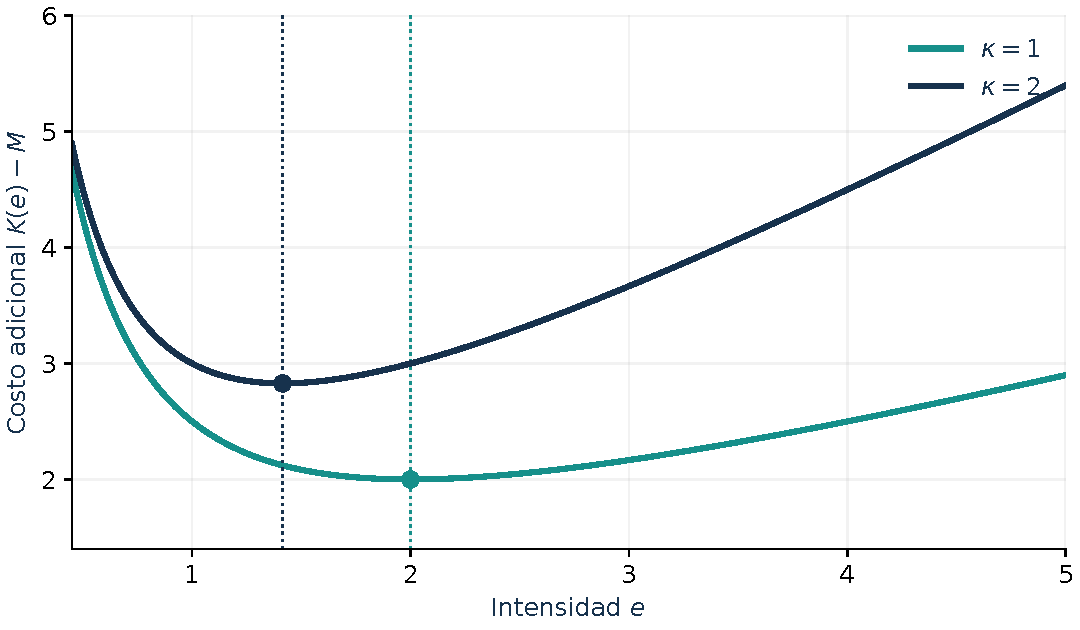
\includegraphics[width=.72\linewidth]{../slides/figures/cost_intensity.pdf}
 \caption{Costo adicional frente a intensidad para $\kappa=1$ y $\kappa=2$, con $M=10$ y $F=2$. Los puntos indican el mínimo de cada curva; fuente: \texttt{code/verify.py}.}\label{fig:costo}
\end{figure}

Para la Figura~\ref{fig:duracion}, $e_0=\sqrt{2F/\bar\kappa}$ y $T_0=1/e_0$ son referencias hipotéticas calculadas con $\bar\kappa$, no con la previsión $\kV$ de un proyecto observado. Las razones representadas obedecen a $e^*/e_0=(\kappa/\bar\kappa)^{-1/2}$ y $T^*/T_0=(\kappa/\bar\kappa)^{1/2}$. Al pasar de la fricción de referencia a la mitad de su valor, la intensidad relativa asciende a $1{,}414$ y la duración cae a $0{,}707$; con una fricción $50\%$ mayor, las razones son $0{,}816$ y $1{,}225$. El valor uno en el centro indica que cada magnitud coincide con su propia referencia, no que fricción, intensidad y duración compartan unidades.
\begin{figure}[htbp]
 \centering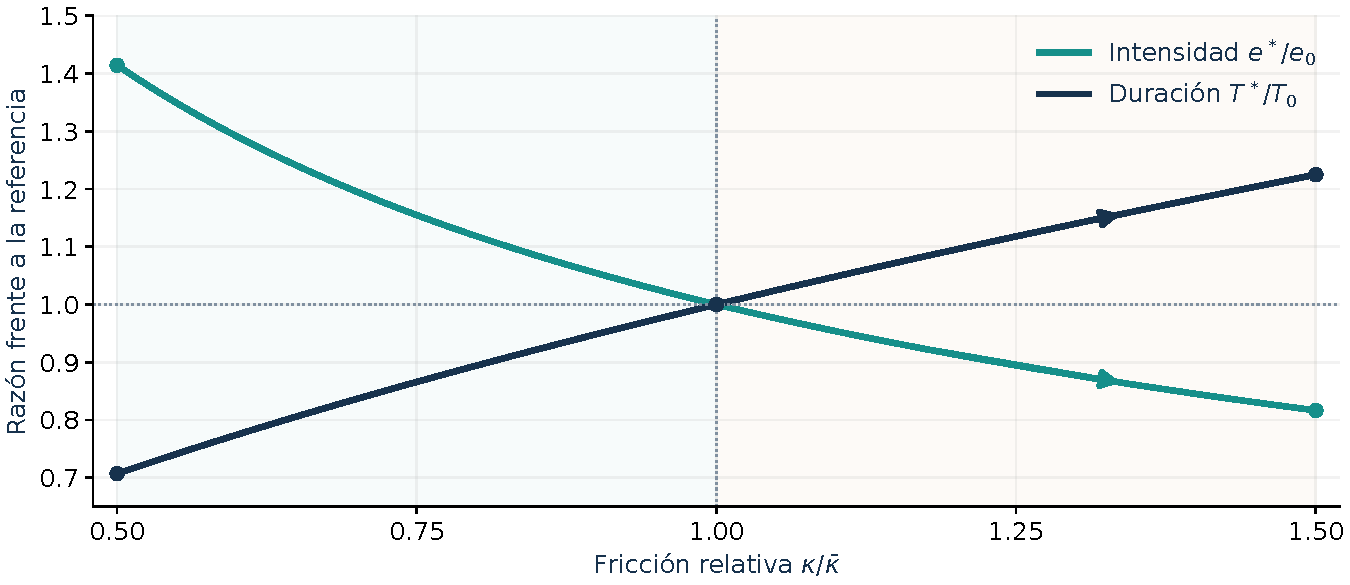
\includegraphics[width=.88\linewidth]{../slides/figures/speed_duration.pdf}
 \caption{Intensidad y duración relativas cuando varía la fricción de un mismo proyecto. La referencia $\bar\kappa=1$ es ilustrativa y no equivale a $\kV$; fuente: \texttt{code/verify.py}.}\label{fig:duracion}
\end{figure}

La Figura~\ref{fig:sobrecosto} compara fricción realizada y previsión según \eqref{eq:lambda}. Si $\kA=1{,}5$ y $\lambda=0$, $\KV=12$ y $\KA\simeq12{,}449$, de modo que $R\simeq0{,}0368>0$; con $\kA=0{,}5$, $\KA\simeq11{,}414$ y $R\simeq-0{,}0500$. Cuando $\lambda=1$, la previsión coincide con la realización y $R=0$ para cualquier $\kA>0$. Los valores son diferencias logarítmicas sin interpretación como puntos porcentuales estimados.
\begin{figure}[htbp]
 \centering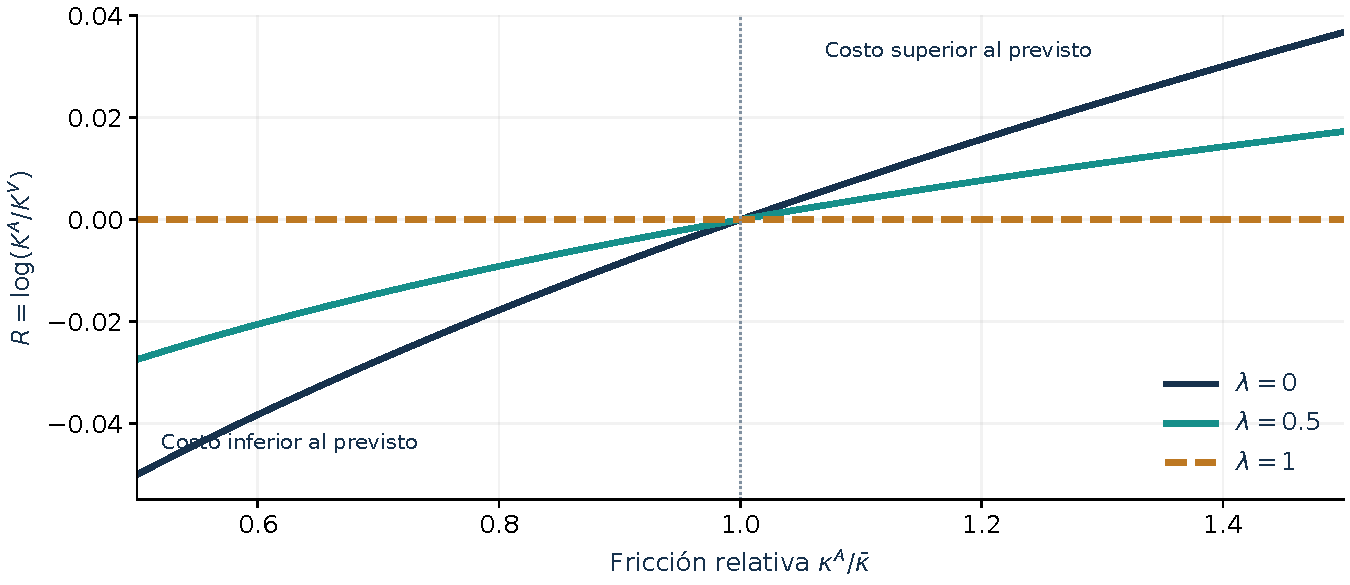
\includegraphics[width=.88\linewidth]{../slides/figures/overrun.pdf}
 \caption{Variación logarítmica de costos al cambiar fricción realizada y anticipación, con $M=10$, $F=2$ y $\bar\kappa=1$. Cada curva mantiene fijo $\lambda\in\{0,0{,}5,1\}$; fuente: \texttt{code/verify.py}.}\label{fig:sobrecosto}
\end{figure}

Las comprobaciones detectan errores algebraicos o de implementación en los casos programados, pero la prueba de las proposiciones es la demostración anterior. Las simulaciones tampoco identifican $\kappa$, $\lambda$ o sus derivadas para distritos peruanos, ni verifican que el alcance de las obras observadas permanezca fijo.

\section{Análisis, verificación crítica y limitaciones}\label{sec:limites}
La restricción principal del resultado distrital es \ref{ass:hetero}. La literatura describe problemas de capacidad, preparación y entorno local, pero no determina que $\kappa_p$ sea positiva o que $\kappa_C$ sea negativa en cada municipio. Además, una municipalidad más pobre puede enfrentar necesidades más urgentes, transferencias distintas u otras prioridades, de modo que una asociación positiva entre pobreza y ejecución presupuestaria, como la documentada por \citet{loayza2014}, no confirma por sí sola el canal específico de intensidad. La Proposición~\ref{prop:uno} entrega signos condicionales del modelo, sin estimación, identificación causal ni validez automática fuera de su dominio.

La Proposición~\ref{prop:dos} utiliza \ref{ass:prevision} para comparar el mismo $M$ y $F$ antes y después. Una modificación de alcance, precios, estándares de calidad o contratos podría elevar el costo aunque la fricción de aceleración no cambiara; tales fenómenos aparecen en \citet{issa2022} y \citet{julca2025}, pero no están modelados por \eqref{eq:signos}. La fecha de referencia también importa: comparar el costo final con la primera estimación puede dar un indicador distinto de compararlo con el monto aprobado cerca del inicio, según ilustra \citet{eliasson2025}. La precisión presupuestaria y el costo de ejecutar son objetos relacionados, aunque conceptualmente distintos.

La correspondencia con indicadores administrativos requiere cautela. El avance financiero dividido entre años desde el primer devengado puede aproximar $e^A=1/T^A$ solo cuando los desembolsos guardan proporción estable con el avance físico y las fechas financieras reflejan el comienzo y el fin reales. Asimismo, el costo actualizado frente al monto viable no es necesariamente $\KA/\KV$: puede incluir adiciones de alcance, revisiones de diseño o registros incompletos. Como el modelo condiciona a culminación, excluir proyectos aún en ejecución puede sesgar la muestra y exige tratar la censura de duración. Se han dejado fuera la decisión de iniciar, una restricción presupuestaria explícita, una trayectoria variable de esfuerzo y la opción de terminar antes por el valor de los beneficios.

La derivación manual de $R_p$ permitió evaluar una afirmación demasiado general que podría surgir de la asistencia de IA: $\kappa_p^A>0$ no garantiza $R_p>0$ si $\kappa^V$ también varía con $p$, tal como muestra \eqref{eq:rp}. El Apéndice~\ref{app:manual} incorpora el manuscrito de esa comprobación y las derivaciones restantes. En la transcripción explicativa se identifica un signo ambiguo en la hoja del costo óptimo y se escribe expresamente la condición correcta $K_e(q;\kappa)=0$. El registro de solicitudes y respuestas pertinentes se conserva en \texttt{prompts.md}; el Apéndice~\ref{app:ia} presenta el veredicto de sus aportes principales. El código simbólico y numérico respalda las identidades implementadas, pero no sustituye la evaluación crítica de supuestos ni la prueba escrita.

La formalización actual de \texttt{lean/Proposition1.lean} declara la positividad de $q=\sqrt{2F/\kappa}$ y que, bajo $M\geq0$, $F>0$ y $\kappa>0$, $q$ es el único mínimo global de $K(e)$ en $e>0$. La prueba se apoya en \eqref{eq:brecha} y, según la comprobación conservada en \texttt{lean/README.md}, compiló sin \texttt{sorry}. Su alcance corresponde solamente a una parte de la Proposición~\ref{prop:uno}: no formaliza aún $T^*$, $K^*$, los signos distritales, la Proposición~\ref{prop:dos} ni la anticipación parcial. Tampoco se ha ejecutado el flujo final de \emph{AppliedModelingLib} sobre un compromiso fijado de este artículo; deberá repetirse después de cerrar el documento y declararse el estado exacto de cada resultado, sin adjudicar a Lean afirmaciones que todavía no verifica.

\section{Conclusión}\label{sec:conclusion}
En un proyecto municipal de trabajo y calidad fijos, la decisión óptima equilibra el gasto por mantener la obra abierta con el costo de acelerar su ejecución. Cuando el gasto por período y la fricción son positivos, una mayor dificultad reduce la intensidad, prolonga la obra y eleva su costo mínimo; sus implicaciones para pobreza y capacidad se mantienen condicionadas a los signos supuestos de la fricción local. Si la previsión y la ejecución comparten alcance, costo base y gasto periódico, la variación del costo es positiva exactamente cuando la fricción realizada supera a la prevista. Esta distinción permite discutir por separado dificultades de implementación y anticipación presupuestaria. Las derivaciones manuscritas se reproducen en el apéndice; su aplicación a obras peruanas aún exige establecer medidas comparables, examinar la heterogeneidad real y distinguir los resultados formalizados en Lean de los que siguen abiertos.

\bibliographystyle{plainnat}
\bibliography{references}
\clearpage
\appendix
\section{Derivaciones manuscritas y guía de lectura}\label{app:manual}
Las cinco hojas manuscritas siguientes reúnen la derivación original de $R_p$ y los pasos restantes del modelo. Las cuatro últimas se conservaron en \texttt{hand/02-derivaciones-manuscritas.pdf}, eliminando únicamente la portada vacía del archivo recibido. Los títulos y la lectura de cada hoja se añaden aquí en texto compuesto para relacionar el trabajo a mano con las ecuaciones del artículo; no sustituyen ni modifican los trazos originales.

\subsection{Trabajo, costo, candidato y unicidad global}
La primera hoja parte del avance físico normalizado $Q=eT=1$ para hallar $T(e)=1/e$, y después integra un gasto constante por período en el intervalo $[0,1/e]$. La condición de primer orden mantiene $M$, $F$ y $\kappa$ fijos y selecciona la raíz positiva $q=\sqrt{2F/\kappa}$. La segunda derivada $2F/e^3>0$ justifica un mínimo local; para demostrar que ese punto existe como mínimo global único se sustituye $F=\kappa q^2/2$ y se completa el cuadrado:
\[
K(e;\kappa)-K(q;\kappa)=\frac{\kappa}{2e}(e-q)^2\geq0,
\quad\text{con igualdad únicamente si }e=q.
\]
El resultado utiliza $e>0$, $F>0$ y $\kappa>0$; $M\geq0$ es un supuesto económico pero se cancela en esta comparación.
\begin{center}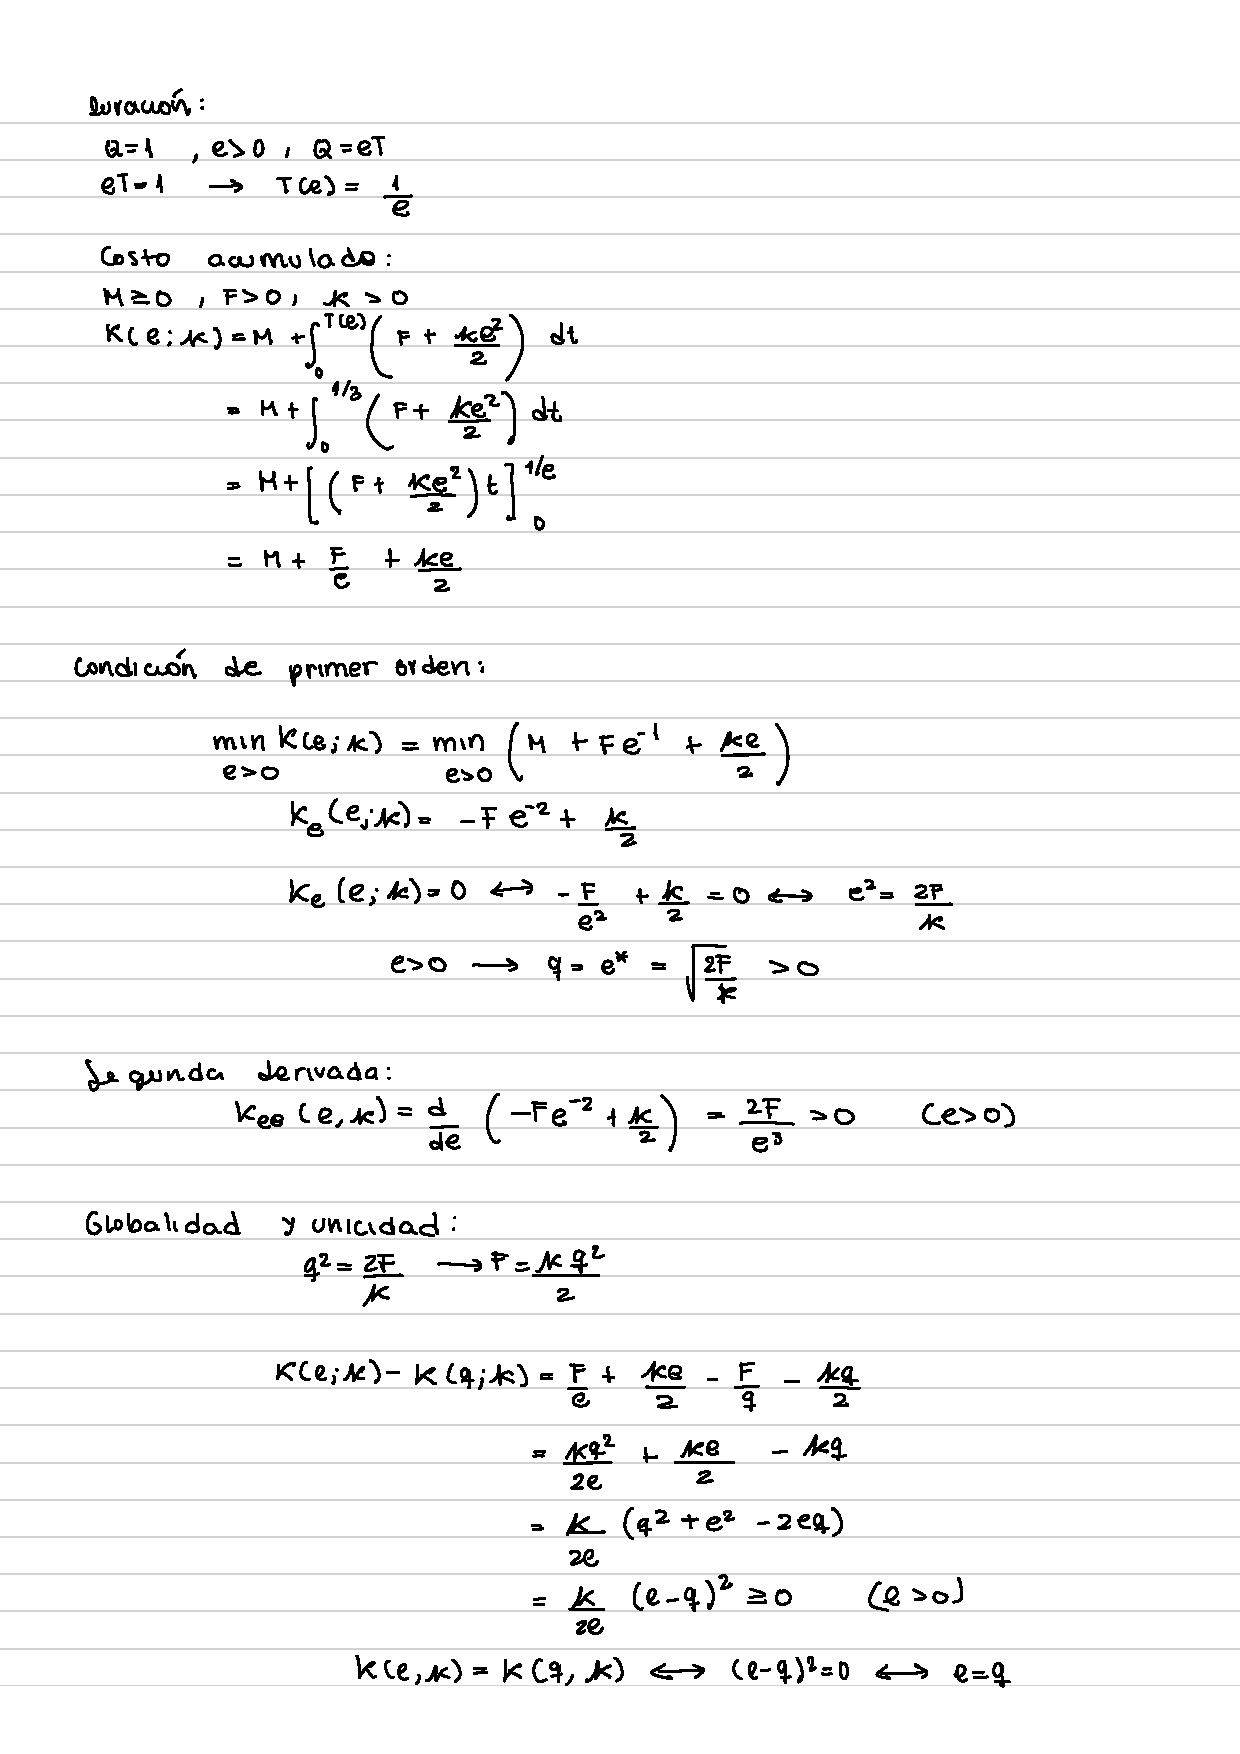
\includegraphics[page=1,width=.96\linewidth,height=.55\textheight,keepaspectratio]{../hand/02-derivaciones-manuscritas.pdf}\end{center}

\clearpage
\subsection{Costo óptimo y signos distritales}
La segunda hoja evalúa $T(q)$ y $K(q;\kappa)$. En el manuscrito, el signo situado entre $K_e(q;\kappa)$ y $0$ puede leerse como una desigualdad; la igualdad que corresponde a la condición de primer orden, y la utilizada en las transformaciones siguientes, es $K_e(q;\kappa)=0$. Al aplicar después la regla de la potencia a $e^*$, $T^*$ y $K^*$ se obtienen signos $(-,+,+)$ respecto de $\kappa$. La regla de la cadena transforma esos signos en los correspondientes a $p$ y $C$, condicionados a $\kappa_p>0$ y $\kappa_C<0$ y a mantener fijos $M$, $F$ y la otra característica distrital.
\begin{center}\includegraphics[page=2,width=.96\linewidth,height=.75\textheight,keepaspectratio]{../hand/02-derivaciones-manuscritas.pdf}\end{center}

\clearpage
\subsection{Tres signos del costo y anticipación parcial}
La tercera hoja aplica la solución óptima dos veces, con $\kV$ en la proyección presupuestaria y $\kA$ al iniciar la ejecución. La cancelación de $M$, el crecimiento estricto de la raíz cuadrada y la monotonía de $\log$ para costos positivos establecen los tres casos de la Proposición~\ref{prop:dos}. Para la extensión, se deriva primero $\kV(\lambda)$ y luego $\KV(\lambda)$; la regla de la cadena para el logaritmo da \eqref{eq:r_lambda}. La comparación requiere el mismo proyecto, alcance, calidad, $M$ y $F$ en ambas etapas.
\begin{center}\includegraphics[page=3,width=.96\linewidth,height=.75\textheight,keepaspectratio]{../hand/02-derivaciones-manuscritas.pdf}\end{center}

\clearpage
\subsection{Convergencia de la previsión y razones de las figuras}
La cuarta hoja usa la identidad $\kA-\kV(\lambda)=(1-\lambda)(\kA-\bar\kappa)$. Para $0\leq\lambda<1$, la Proposición~\ref{prop:dos} fija el signo de $R$; en $\lambda=1$, la coincidencia de las fricciones implica $R=0$, mientras $e^A$ y $\KA$ permanecen constantes. Las razones de intensidad y duración dividen cada solución entre su propia referencia hipotética $e_0$ o $T_0$, calculada con $\bar\kappa$. Esa referencia de la simulación no es la fricción presupuestada $\kV$.
\begin{center}\includegraphics[page=4,width=.96\linewidth,height=.72\textheight,trim=0 350 0 0,clip,keepaspectratio]{../hand/02-derivaciones-manuscritas.pdf}\end{center}

\clearpage
\subsection{Revisión independiente de la derivada respecto de la pobreza}
La hoja anterior de la autora diferencia ambos logaritmos en $R(p)$ mediante la regla de la cadena, de donde $R_p=(\KA)_p/\KA-(\KV)_p/\KV$. Su veredicto es que $\kappa_p^A>0$ por sí sola no determina el signo de $R_p$ cuando $\kappa_p^V$ también puede variar. Si $\kappa_p^V=0$, la positividad de $\kappa_p^A$ sí da $R_p>0$. Así se examina una conclusión demasiado fuerte que podría atribuirse a la asistencia de IA.
\begin{center}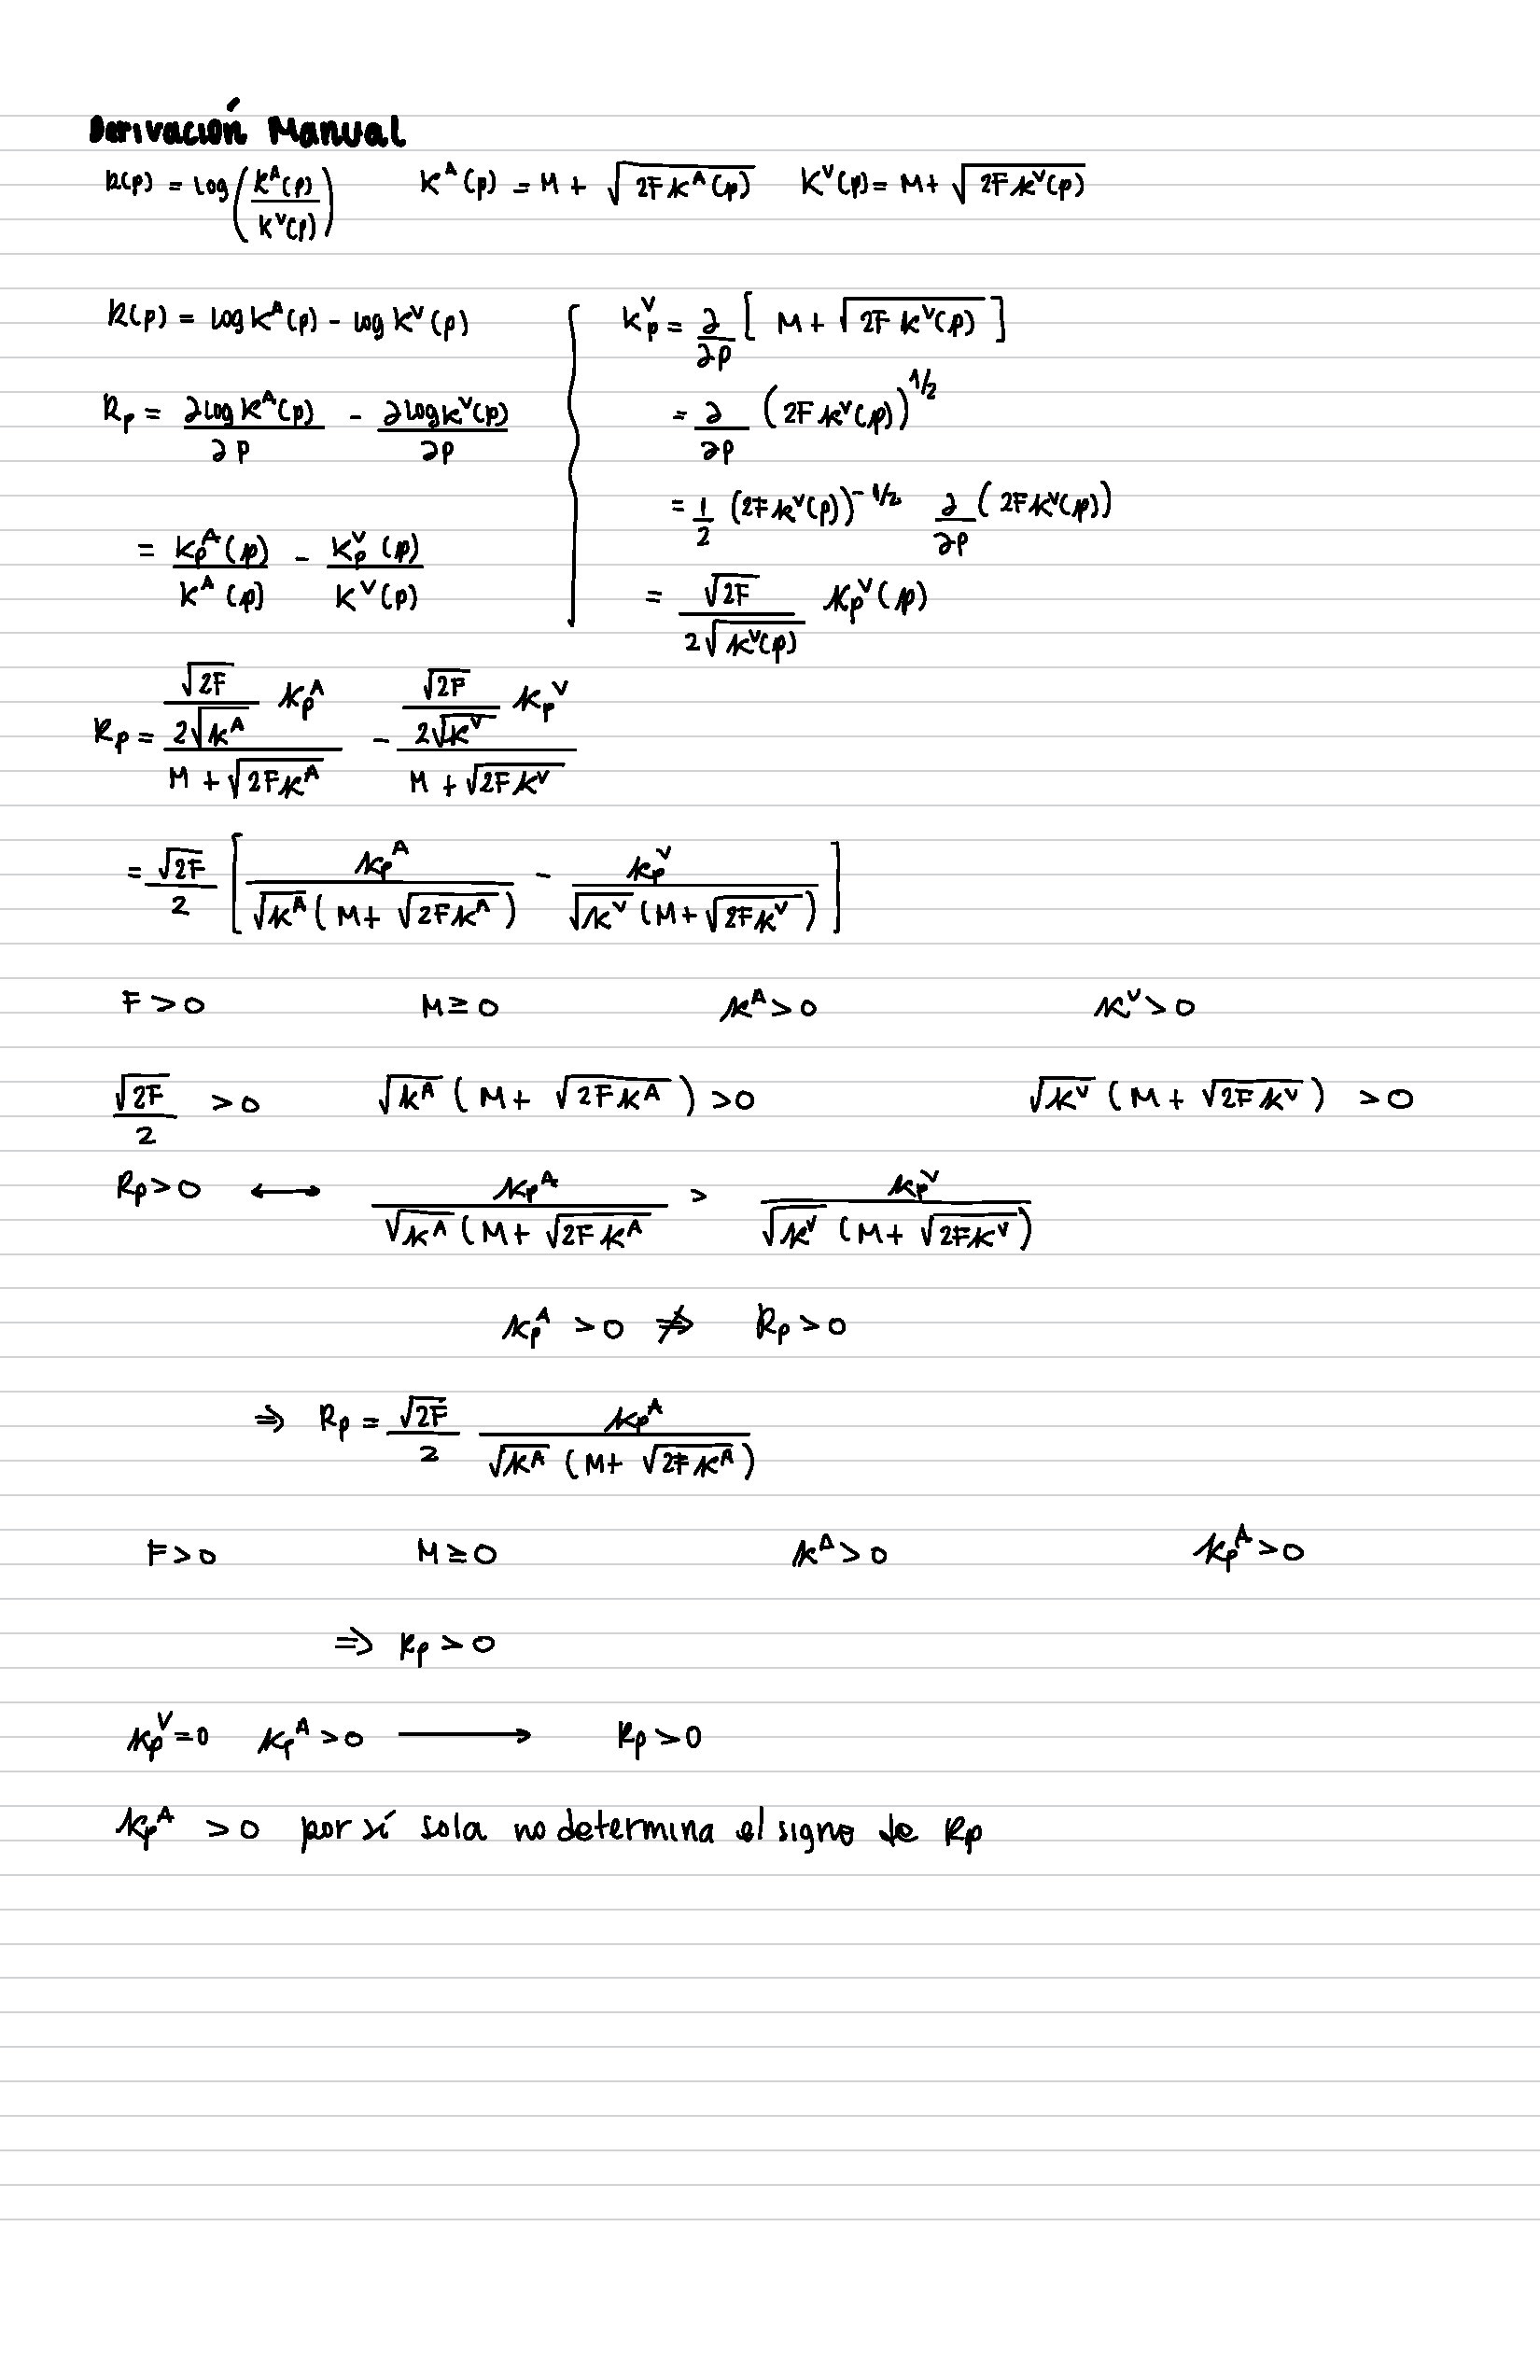
\includegraphics[page=1,width=.96\linewidth,height=.75\textheight,keepaspectratio]{../hand/01-derivacion-manual-Rp.pdf}\end{center}

\clearpage
\section{Correspondencia con la formalización Lean}\label{app:lean}
La formalización disponible se corresponde con la versión del artículo indicada en \texttt{lean/README.md}. Una compilación anterior del archivo \texttt{Proposition1.lean} verificó el mínimo global único; la ejecución del flujo de contribución y las declaraciones de los demás resultados están pendientes de comprobación. La tabla no atribuye a Lean los signos distritales ni el resultado sobre sobrecostos.
\begin{center}
\small
\begin{tabular}{p{.21\linewidth}p{.34\linewidth}p{.34\linewidth}}
\toprule
Resultado del artículo & Declaración y archivo Lean & Estado y alcance \\
\midrule
Proposición 1 & \texttt{MunicipalProject.}\newline\texttt{unique\_global\_minimum} en \texttt{lean/Proposition1.lean} & Mínimo global único compilado anteriormente; duración, costo y signos abiertos. \\
Proposición 2 & --- & Abierta: falta formalizar la equivalencia de los tres signos. \\
Extensión de anticipación & --- & Abierta: falta formalizar $R_\lambda$ y el caso $R(1)=0$. \\
\bottomrule
\end{tabular}
\end{center}


\clearpage
\section{Evaluación de la colaboración con IA}\label{app:ia}
El archivo \texttt{prompts.md} conserva las consultas y respuestas pertinentes en bruto. La tabla separa lo sugerido durante esa colaboración de lo que se admite como resultado de este artículo; el criterio de aceptación es la coincidencia con las hipótesis escritas y la comprobación independiente, no la fluidez de una respuesta.
\begin{center}
\small
\begin{tabular}{p{.21\linewidth}p{.31\linewidth}p{.37\linewidth}}
\toprule
Contribución examinada & Veredicto y razón & Verificación \\
\midrule
Óptimo de intensidad y costo & Aceptada con $F,\kappa>0$ y $e>0$. La condición de primer orden sola no demuestra globalidad. & Identidad cuadrática \eqref{eq:brecha} en el artículo y manuscrito; sustituciones en SymPy y comparación en 3000 casos. \\
Signos distritales & Condicionales, no estimaciones: los signos de $\kappa_p$ y $\kappa_C$ son supuestos estructurales. & Regla de la cadena y manuscrito; contraste de su interpretación con los resultados de \citet{loayza2014}. \\
Sobrecosto siempre que la fricción sea elevada & Rechazada. El nivel absoluto de $\kA$ no fija la diferencia respecto de la previsión. & Resta de costos y tres equivalencias de la Proposición~\ref{prop:dos}; casos positivos, negativos e iguales en \texttt{code/verify.py}. \\
$\kappa_p^A>0$ bastaría para $R_p>0$ & Rechazada si $\kappa_p^V$ puede variar. Ambas derivadas de costos entran en $R_p$. & Hoja manuscrita propia y ecuación \eqref{eq:rp}; comprobación simbólica del código. \\
Mejor anticipación abarata la ejecución & Rechazada bajo la extensión propuesta: $\lambda$ mueve el costo previsto, no $\KA$ con $\kA$ fija. & Derivada \eqref{eq:r_lambda}, límite $R(1)=0$, manuscrito y valores del script. \\
\bottomrule
\end{tabular}
\end{center}
Esta evaluación se limita a las identidades y condiciones de este modelo. La revisión de fuentes literarias y su correspondencia con obras municipales requieren juicio sobre unidades de análisis y sobre el momento en que se fija cada presupuesto; ninguna comprobación algebraica decide esas cuestiones por sí sola.

\end{document}
